%2multibyte Version: 5.50.0.2960 CodePage: 65001
% ------------------------------------------------------------
% Macro matematiche ufficiali del progetto MQF
% Coerenti con MQF_Notazione.tex
% ------------------------------------------------------------
% Fallback utile per compilazione esterna se qualche titolo resta scritto come \QTR.
% Scientific WorkPlace usa \QTR internamente; in Beamer \QTR{frametitle}{Titolo}
% deve espandersi in \frametitle{Titolo}.

\documentclass[handout]{beamer}%
\usepackage{mathpazo}
%\usepackage{hyperref}
\usepackage{multimedia}
\usepackage{amsmath}
\usepackage{amsfonts}
\usepackage{amssymb}
\usepackage{graphicx}%
\setcounter{MaxMatrixCols}{30}
%TCIDATA{OutputFilter=latex2.dll}
%TCIDATA{Version=5.50.0.2960}
%TCIDATA{Codepage=65001}
%TCIDATA{CSTFile=beamer.cst}
%TCIDATA{Created=Saturday, May 16, 2026 09:09:59}
%TCIDATA{LastRevised=Saturday, May 16, 2026 11:24:58}
%TCIDATA{<META NAME="GraphicsSave" CONTENT="32">}
%TCIDATA{<META NAME="SaveForMode" CONTENT="2">}
%TCIDATA{BibliographyScheme=Manual}
%TCIDATA{<META NAME="DocumentShell" CONTENT="Other Documents\SW\Slides - Beamer">}
%BeginMSIPreambleData
\providecommand{\U}[1]{\protect\rule{.1in}{.1in}}
%EndMSIPreambleData
\newenvironment{stepenumerate}{\begin{enumerate}[<+->]}{\end{enumerate}}
\newenvironment{stepitemize}{\begin{itemize}[<+->]}{\end{itemize} }
\newenvironment{stepenumeratewithalert}{\begin{enumerate}[<+-| alert@+>]}{\end{enumerate}}
\newenvironment{stepitemizewithalert}{\begin{itemize}[<+-| alert@+>]}{\end{itemize} }
\usetheme{Madrid}
\setbeamersize{, text margin right=5mm}
\providecommand{\R}{\mathbb{R}}
\providecommand{\N}{\mathbb{N}}
\providecommand{\E}{\mathbb{E}}
\providecommand{\Prob}{\mathbb{P}}
\providecommand{\Q}{\mathbb{Q}}
\providecommand{\F}{\mathcal{F}}
\providecommand{\B}{\mathcal{B}}
\providecommand{\G}{\mathcal{G}}
\providecommand{\Var}{\operatorname{Var}}
\providecommand{\Cov}{\operatorname{Cov}}
\providecommand{\VaR}{\operatorname{VaR}}
\providecommand{\CVaR}{\operatorname{CVaR}}
\providecommand{\argmin}{\operatorname*{arg\,min}}
\providecommand{\argmax}{\operatorname*{arg\,max}}
\providecommand{\EVPI}{\operatorname{EVPI}}
\providecommand{\VSS}{\operatorname{VSS}}
\providecommand{\QTR}[2]{\csname #1\endcsname{#2}}
%BeginMSIPreambleData
\ifx\pdfoutput\relax\let\pdfoutput=\undefined\fi
\newcount\msipdfoutput
\ifx\pdfoutput\undefined\else
\ifcase\pdfoutput\else
\msipdfoutput=1
\ifx\paperwidth\undefined\else
\ifdim\paperheight=0pt\relax\else\pdfpageheight\paperheight\fi
\ifdim\paperwidth=0pt\relax\else\pdfpagewidth\paperwidth\fi
\fi\fi\fi
%EndMSIPreambleData


\title{Lezione 2 - Variabili casuali}
\subtitle{Metodi Quantitativi per la Finanza}
\author[P. Falbo, C. Pelizzari]{{\LARGE Paolo Falbo, Cristian Pelizzari}}
\institute[]{{\large Dipartimento Economia e Management}}
\date[]{}
\titlegraphic{

\includegraphics[width=3.3cm]{graphics/logo-Unibs-esteso.png}
}

\begin{document}
\maketitle

\section{Apertura}

%***********************************
\subsection{Apertura: perch\'{e} servono le variabili casuali}

%TCIMACRO{\TeXButton{BeginFrame}{\begin{frame}}}%
%BeginExpansion
\begin{frame}%
%EndExpansion

\QTR{frametitle}{Variabili casuali: dagli scenari ai valori}

\textbf{Idea centrale.}

\medskip

L'incertezza finanziaria diventa operativa quando agli scenari associamo
grandezze numeriche.

\[
\omega\in\Omega
\quad\longmapsto\quad
X(\omega)\in\mathbb{R}
\]

\medskip

\textbf{Esempi finanziari.}

\[
\begin{array}{rcl}
R   & = & \mbox{rendimento aleatorio},\\[4pt]
L   & = & \mbox{perdita aleatoria},\\[4pt]
S_T & = & \mbox{prezzo futuro aleatorio},\\[4pt]
H   & = & \mbox{payoff aleatorio}.
\end{array}
\]

\medskip

Gli eventi restano il fondamento probabilistico; la finanza quantitativa lavora
sui valori numerici generati dagli scenari.

%TCIMACRO{\TeXButton{Transition: Box Out}{\transboxout}}%
%BeginExpansion
\transboxout%
%EndExpansion
%TCIMACRO{\TeXButton{EndFrame}{\end{frame}}}%
%BeginExpansion
\end{frame}%
%EndExpansion


%***********************************
\subsection{La domanda del capitolo}

%TCIMACRO{\TeXButton{BeginFrame}{\begin{frame}}}%
%BeginExpansion
\begin{frame}%
%EndExpansion

\QTR{frametitle}{La domanda del capitolo}

Non basta chiedere se un evento si verifica: occorre descrivere la
distribuzione dei valori assunti da una grandezza finanziaria aleatoria.

\[
\Prob(R<0),
\qquad
\Prob(L>\ell),
\qquad
\Prob(S_T>K)
\]

\medskip

\textbf{Domanda guida.}

\medskip

Come si descrive probabilisticamente un rendimento, una perdita o un payoff
aleatorio?

\medskip

\[
\begin{array}{rcl}
R   & : & \mbox{rendimento futuro},\\[4pt]
L   & : & \mbox{perdita di portafoglio},\\[4pt]
S_T & : & \mbox{prezzo futuro del sottostante},\\[4pt]
H   & : & \mbox{payoff di un contratto finanziario}.
\end{array}
\]

%TCIMACRO{\TeXButton{Transition: Box Out}{\transboxout}}%
%BeginExpansion
\transboxout%
%EndExpansion
%TCIMACRO{\TeXButton{EndFrame}{\end{frame}}}%
%BeginExpansion
\end{frame}%
%EndExpansion


%***********************************
\subsection{Mappa del capitolo}

%TCIMACRO{\TeXButton{BeginFrame}{\begin{frame}}}%
%BeginExpansion
\begin{frame}%
%EndExpansion

\QTR{frametitle}{Mappa del capitolo}

Il capitolo costruisce il ponte tra probabilit\`{a} astratta e misurazione
quantitativa del rischio.

\[
(\Omega,\F,\Prob)
\quad\longrightarrow\quad
X
\quad\longrightarrow\quad
\Prob_X,\ F_X,\ p_X,\ f_X
\quad\longrightarrow\quad
\E[X],\ \Var(X),\ q_\alpha(X)
\]

\medskip

\[
\begin{array}{rcl}
\Prob_X & : & \mbox{distribuzione indotta da } X,\\[4pt]
F_X     & : & \mbox{funzione di distribuzione},\\[4pt]
p_X     & : & \mbox{funzione di probabilit\`{a}},\\[4pt]
f_X     & : & \mbox{densit\`{a} di probabilit\`{a}},\\[4pt]
\E[X],\ \Var(X),\ q_\alpha(X)
        & : & \mbox{sintesi di posizione, dispersione e coda}.
\end{array}
\]

\medskip

Obiettivo: tradurre l'incertezza sugli scenari in strumenti operativi per
rendimenti, perdite, payoff e rischio di coda.

%TCIMACRO{\TeXButton{Transition: Box Out}{\transboxout}}%
%BeginExpansion
\transboxout%
%EndExpansion
%TCIMACRO{\TeXButton{EndFrame}{\end{frame}}}%
%BeginExpansion
\end{frame}%
%EndExpansion

%***********************************
\subsection{Definizione di variabile casuale}

%TCIMACRO{\TeXButton{BeginFrame}{\begin{frame}}}%
%BeginExpansion
\begin{frame}%
%EndExpansion

\QTR{frametitle}{Variabile casuale: definizione}

Una variabile casuale reale associa un numero reale a ciascun esito dello spazio
campionario.

\[
X:\Omega\longrightarrow\mathbb{R}
\]

\medskip

Se $\omega\in\Omega$ \`{e} uno scenario, allora $X(\omega)$ \`{e} il valore
numerico generato da quello scenario.

\medskip

\[
\begin{array}{rcl}
\omega & : & \mbox{scenario possibile},\\[4pt]
X(\omega) & : & \mbox{valore della grandezza aleatoria nello scenario } \omega.
\end{array}
\]

\medskip

Esempi: rendimento futuro, perdita di portafoglio, prezzo futuro, payoff.

%TCIMACRO{\TeXButton{Transition: Box Out}{\transboxout}}%
%BeginExpansion
\transboxout%
%EndExpansion
%TCIMACRO{\TeXButton{EndFrame}{\end{frame}}}%
%BeginExpansion
\end{frame}%
%EndExpansion


%***********************************
\subsection{Eventi generati da una variabile casuale}

%TCIMACRO{\TeXButton{BeginFrame}{\begin{frame}}}%
%BeginExpansion
\begin{frame}%
%EndExpansion

\QTR{frametitle}{Eventi generati da una variabile casuale}

\textbf{Una condizione sui valori di $X$ individua un insieme di scenari}.

\[
\{X\leq x\}
=
\{\omega\in\Omega:X(\omega)\leq x\}
\]

\medskip

Analogamente,

\[
\{X=x_i\}
=
\{\omega\in\Omega:X(\omega)=x_i\},
\]

\[
\{a<X\leq b\}
=
\{\omega\in\Omega:a<X(\omega)\leq b\}.
\]

\medskip

La probabilit\`{a} resta assegnata a eventi dello spazio originario:

\[
\Prob(X\leq x)
=
\Prob(\{\omega\in\Omega:X(\omega)\leq x\}).
\]

%TCIMACRO{\TeXButton{Transition: Box Out}{\transboxout}}%
%BeginExpansion
\transboxout%
%EndExpansion
%TCIMACRO{\TeXButton{EndFrame}{\end{frame}}}%
%BeginExpansion
\end{frame}%
%EndExpansion


%***********************************
\subsection{Misurabilit\`{a}}

%TCIMACRO{\TeXButton{BeginFrame}{\begin{frame}}}%
%BeginExpansion
\begin{frame}%
%EndExpansion

\QTR{frametitle}{La condizione di misurabilit\`{a}}

Una funzione $X:\Omega\to\mathbb{R}$ \`{e} una variabile casuale \textbf{misurabile} se gli eventi
del tipo $\{X\leq x\}$ sono inclusi nella $\sigma$-algebra $\F$, (famiglia degli eventi rilevanti).

\[
\{X\leq x\}\in\F
\qquad
\mbox{per ogni } x\in\mathbb{R}.
\]

\medskip

Questa condizione garantisce che la quantit\`{a}

\[
\Prob(X\leq x)
\]

sia ben definita.

\medskip

\[
\begin{array}{rcl}
X & : & \mbox{assegna valori numerici agli esiti},\\[4pt]
\F & : & \mbox{contiene gli eventi rilevanti / osservabili},\\[4pt]
\Prob & : & \mbox{assegna probabilit\`{a} agli eventi di } \F.
\end{array}
\]

%TCIMACRO{\TeXButton{Transition: Box Out}{\transboxout}}%
%BeginExpansion
\transboxout%
%EndExpansion
%TCIMACRO{\TeXButton{EndFrame}{\end{frame}}}%
%BeginExpansion
\end{frame}%
%EndExpansion

%***********************************
\subsection{Esempio guida: scenari, regimi e rendimento}

%TCIMACRO{\TeXButton{BeginFrame}{\begin{frame}}}%
%BeginExpansion
\begin{frame}%
%EndExpansion

\QTR{frametitle}{Sei scenari, tre regimi di mercato}

Consideriamo sei esiti elementari:

\[
\Omega=\{\omega_1,\omega_2,\omega_3,\omega_4,\omega_5,\omega_6\}.
\]

\medskip

Gli scenari sono raggruppati in tre regimi di mercato:

\[
A_1=\{\omega_1,\omega_2\},
\qquad
A_2=\{\omega_3,\omega_4\},
\qquad
A_3=\{\omega_5,\omega_6\}.
\]

\medskip

\[
\begin{array}{rcl}
A_1 & : & \mbox{regime sfavorevole},\\[4pt]
A_2 & : & \mbox{regime intermedio},\\[4pt]
A_3 & : & \mbox{regime favorevole}.
\end{array}
\]

\medskip

Idea: il modello distingue i regimi, non necessariamente ogni singolo esito
elementare.

%TCIMACRO{\TeXButton{Transition: Box Out}{\transboxout}}%
%BeginExpansion
\transboxout%
%EndExpansion
%TCIMACRO{\TeXButton{EndFrame}{\end{frame}}}%
%BeginExpansion
\end{frame}%
%EndExpansion


%***********************************
\subsection{Sigma-algebra generata dalla partizione}

%TCIMACRO{\TeXButton{BeginFrame}{\begin{frame}}}%
%BeginExpansion
\begin{frame}%
%EndExpansion

\QTR{frametitle}{Eventi osservabili nel modello}

La partizione genera la sigma-algebra degli eventi osservabili:

\[
\F=\sigma(A_1,A_2,A_3).
\]

\medskip

Esplicitamente,

\[
\F=
\{\varnothing,
A_1,A_2,A_3,
A_1\cup A_2,A_1\cup A_3,A_2\cup A_3,
\Omega\}.
\]

\medskip

Gli eventi ammissibili sono le unioni dei blocchi della partizione.

\medskip

\[
\begin{array}{rcl}
A_1\cup A_2 & : & \mbox{regime non favorevole},\\[4pt]
A_2\cup A_3 & : & \mbox{regime non sfavorevole},\\[4pt]
\Omega      & : & \mbox{evento certo}.
\end{array}
\]

\medskip

La sigma-algebra specifica quali eventi sono descrivibili nel modello.

%TCIMACRO{\TeXButton{Transition: Box Out}{\transboxout}}%
%BeginExpansion
\transboxout%
%EndExpansion
%TCIMACRO{\TeXButton{EndFrame}{\end{frame}}}%
%BeginExpansion
\end{frame}%
%EndExpansion


%***********************************
\subsection{Rendimento come variabile casuale}

%TCIMACRO{\TeXButton{BeginFrame}{\begin{frame}}}%
%BeginExpansion
\begin{frame}%
%EndExpansion

\QTR{frametitle}{Il rendimento come funzione degli scenari}

Definiamo una variabile casuale $X$ che rappresenta il rendimento del
portafoglio:

\[
X(\omega)=
\begin{cases}
-0.04, & \mbox{se } \omega\in A_1,\\
 0.01, & \mbox{se } \omega\in A_2,\\
 0.06, & \mbox{se } \omega\in A_3.
\end{cases}
\]

\medskip

La variabile casuale aggrega scenari diversi nello stesso valore numerico:

\[
\begin{array}{rcl}
\{X=-0.04\} = A_1, \qquad
\{X=0.01\}  = A_2,\qquad
\{X=0.06\}  = A_3.
\end{array}
\]

\medskip

Esempi di eventi generati da $X$:

\[
\{X<0\}=A_1,
\qquad
\{X\geq 0.01\}=A_2\cup A_3.
\]

\medskip

La condizione numerica su $X$ individua un evento appartenente a $\F$.

%TCIMACRO{\TeXButton{Transition: Box Out}{\transboxout}}%
%BeginExpansion
\transboxout%
%EndExpansion
%TCIMACRO{\TeXButton{EndFrame}{\end{frame}}}%
%BeginExpansion
\end{frame}%
%EndExpansion

%***********************************
\subsection{Controimmagini, Borel e distribuzione indotta}

%TCIMACRO{\TeXButton{BeginFrame}{\begin{frame}}}%
%BeginExpansion
\begin{frame}%
%EndExpansion

\QTR{frametitle}{Controimmagini: dai valori agli eventi}

Sia $X:\Omega\to\mathbb{R}$ una funzione e sia $B\subseteq\mathbb{R}$.

\medskip

La controimmagine di $B$ mediante $X$ \`{e}

\[
X^{-1}(B)=\{\omega\in\Omega:X(\omega)\in B\}.
\]

\medskip

Essa \`{e} un sottoinsieme di $\Omega$, quindi un candidato evento.

\medskip

Esempi:

\[
X^{-1}((-\infty,x])
=
\{\omega\in\Omega:X(\omega)\leq x\}
=
\{X\leq x\},
\]

\[
X^{-1}((a,b])
=
\{\omega\in\Omega:a<X(\omega)\leq b\}
=
\{a<X\leq b\}.
\]

\medskip

(la notazione $X^{-1}(B)$ non è da intendersi nel senso abituale, ma come mappa che lavora in direzione inversa alla v.c. $X$).

%TCIMACRO{\TeXButton{Transition: Box Out}{\transboxout}}%
%BeginExpansion
\transboxout%
%EndExpansion
%TCIMACRO{\TeXButton{EndFrame}{\end{frame}}}%
%BeginExpansion
\end{frame}%
%EndExpansion


%***********************************
\subsection{Il ruolo della sigma-algebra boreliana}

%TCIMACRO{\TeXButton{BeginFrame}{\begin{frame}}}%
%BeginExpansion
\begin{frame}%
%EndExpansion

\QTR{frametitle}{Il ruolo di $\mathcal{B}(\mathbb{R})$}

Per variabili casuali reali, gli eventi sui valori di $X$ sono sottoinsiemi
della retta reale.

\medskip

La classe naturale di tali insiemi \`{e} la sigma-algebra boreliana:

\[
\mathcal{B}(\mathbb{R}).
\]

\medskip

Essa contiene gli insiemi normalmente usati per descrivere eventi sui valori
reali:

\[
(-\infty,x],
\qquad
(a,b],
\qquad
[a,b],
\qquad
(x,+\infty).
\]

\medskip

La misurabilit\`{a} richiede:

\[
B\in\mathcal{B}(\mathbb{R})
\quad\Longrightarrow\quad
X^{-1}(B)\in\F.
\]

\medskip

Quindi ogni condizione boreliana sui valori di $X$ genera un evento osservabile
nello spazio originario.

%TCIMACRO{\TeXButton{Transition: Box Out}{\transboxout}}%
%BeginExpansion
\transboxout%
%EndExpansion
%TCIMACRO{\TeXButton{EndFrame}{\end{frame}}}%
%BeginExpansion
\end{frame}%
%EndExpansion


%***********************************
\subsection{Distribuzione indotta}

%TCIMACRO{\TeXButton{BeginFrame}{\begin{frame}}}%
%BeginExpansion
\begin{frame}%
%EndExpansion

\QTR{frametitle}{Distribuzione indotta da una variabile casuale}

La variabile casuale $X$ \textbf{trasferisce} o \textbf{induce} la probabilit\`{a} da $\Omega$ alla retta reale. Ciò è possibile grazie alla \textbf{misura di probabilit\`{a} indotta} $\Prob_X$: 
\[
\Prob_X:=\Prob\circ X^{-1} 
\]
ossia, per ogni $B \in\mathcal{B}(\mathbb{R})$
\[
\Prob_X(B) = \Prob\left(X^{-1}(B)\right).
\]
con la differenza che
\[
\begin{array}{ccc}
B\subseteq\mathbb{R}
& \longmapsto &
X^{-1}(B)\subseteq\Omega\\[5pt]
\mbox{insieme di valori}
& &
\mbox{evento nello spazio campionario}
\end{array}
\]

\[
\begin{array}{rcl}
\Prob     & : & \mbox{probabilit\`{a} sugli eventi di } \Omega,\\[4pt]
\Prob_X  & : & \mbox{probabilit\`{a} indotta sui valori reali di } X.
\end{array}
\]

\medskip

Messaggio: la misura $\Prob_X$ è importante perché costituisce la \textbf{distribuzione} di $X$, cioè la collezione delle  probabilit\`{a} di tutti i possibili eventi $\{X\in B\}$.

%TCIMACRO{\TeXButton{Transition: Box Out}{\transboxout}}%
%BeginExpansion
\transboxout%
%EndExpansion
%TCIMACRO{\TeXButton{EndFrame}{\end{frame}}}%
%BeginExpansion
\end{frame}%
%EndExpansion

%***********************************
\subsection{Funzione di distribuzione}

%TCIMACRO{\TeXButton{BeginFrame}{\begin{frame}}}%
%BeginExpansion
\begin{frame}%
%EndExpansion

\QTR{frametitle}{Funzione di distribuzione}

La distribuzione di una variabile casuale reale pu\`{o} essere rappresentata
mediante la funzione di distribuzione.

\[
F_X(x)
=
\Prob_X((-\infty,x])
=
\Prob(X\leq x),
\qquad x\in\mathbb{R}.
\]

\medskip

$F_X(x)$ misura la probabilit\`{a} cumulata fino alla soglia $x$.

\medskip

\[
\begin{array}{rcl}
x & : & \mbox{soglia reale},\\[4pt]
\{X\leq x\} & : & \mbox{evento generato dalla soglia},\\[4pt]
F_X(x) & : & \mbox{probabilit\`{a} cumulata fino a } x.
\end{array}
\]

\medskip

Messaggio: $F_X$ traduce la distribuzione di $X$ in una funzione reale di
variabile reale.

%TCIMACRO{\TeXButton{Transition: Box Out}{\transboxout}}%
%BeginExpansion
\transboxout%
%EndExpansion
%TCIMACRO{\TeXButton{EndFrame}{\end{frame}}}%
%BeginExpansion
\end{frame}%
%EndExpansion


%***********************************
\subsection{Propriet\`{a} della funzione di distribuzione}

%TCIMACRO{\TeXButton{BeginFrame}{\begin{frame}}}%
%BeginExpansion
\begin{frame}%
%EndExpansion

\QTR{frametitle}{Propriet\`{a} fondamentali di $F_X$}

Per ogni variabile casuale reale, la funzione di distribuzione soddisfa:

\[
0\leq F_X(x)\leq 1,
\qquad x\in\mathbb{R}.
\]

\[
x_1\leq x_2
\quad\Longrightarrow\quad
F_X(x_1)\leq F_X(x_2).
\]

\[
\lim_{x\to -\infty}F_X(x)=0,
\qquad
\lim_{x\to +\infty}F_X(x)=1.
\]

\medskip

Inoltre, $F_X$ \`{e} continua da destra:

\[
\lim_{h\downarrow 0}F_X(x+h)=F_X(x).
\]

\medskip
\textbf{Traduzione colloquiale}: se $F_x$ fa un salto, il nuovo scalino possiede il primo punto, il vecchio scalino invece non ha ultimo punto. 

%TCIMACRO{\TeXButton{Transition: Box Out}{\transboxout}}%
%BeginExpansion
\transboxout%
%EndExpansion
%TCIMACRO{\TeXButton{EndFrame}{\end{frame}}}%
%BeginExpansion
\end{frame}%
%EndExpansion


%***********************************
\subsection{Probabilit\`{a} di intervallo e salti}

%TCIMACRO{\TeXButton{BeginFrame}{\begin{frame}}}%
%BeginExpansion
\begin{frame}%
%EndExpansion

\QTR{frametitle}{Intervalli, limite sinistro e salti}

La funzione di distribuzione consente di calcolare probabilit\`{a} di intervallo:

\[
\Prob_X(a<X\leq b)
=
F_X(b)-F_X(a),
\qquad a<b.
\]

\medskip

Per trattare disuguaglianze strette si usa il limite sinistro:

\[
F_X(x^-)
=
\lim_{h\downarrow 0}F_X(x-h).
\]

\[
\Prob(X<x)=F_X(x^-).
\]

\medskip

La probabilit\`{a} puntuale \`{e} l'ampiezza del salto di $F_X$:

\[
\Prob_X(X=x)
=
F_X(x)-F_X(x^-).
\]

\medskip

Messaggio: un salto della funzione di distribuzione corrisponde a probabilit\`{a}
positiva assegnata a un singolo valore.

%TCIMACRO{\TeXButton{Transition: Box Out}{\transboxout}}%
%BeginExpansion
\transboxout%
%EndExpansion
%TCIMACRO{\TeXButton{EndFrame}{\end{frame}}}%
%BeginExpansion
\end{frame}%
%EndExpansion

%***********************************
\subsection{Funzione di distribuzione discreta}

%TCIMACRO{\TeXButton{BeginFrame}{\begin{frame}}}%
%BeginExpansion
\begin{frame}%
%EndExpansion

\QTR{frametitle}{Funzione di distribuzione: caso discreto}

Nel caso discreto, la funzione di distribuzione \`{e} una funzione a gradini.

\medskip

Per l'esempio guida:

\[
\begin{array}{c|ccc}
x & -0.04 & 0.01 & 0.06\\
\hline
p_X(x) & 0.25 & 0.50 & 0.25
\end{array}
\]

\[
F_X(x)=
\begin{cases}
0, & x<-0.04,\\
0.25, & -0.04\leq x<0.01,\\
0.75, & 0.01\leq x<0.06,\\
1, & x\geq 0.06.
\end{cases}
\]

\medskip

I salti di $F_X$ coincidono con le probabilit\`{a} puntuali $p_X(x)$.

%TCIMACRO{\TeXButton{Transition: Box Out}{\transboxout}}%
%BeginExpansion
\transboxout%
%EndExpansion
%TCIMACRO{\TeXButton{EndFrame}{\end{frame}}}%
%BeginExpansion
\end{frame}%
%EndExpansion


%***********************************
\subsection{Grafico della funzione di distribuzione}

%TCIMACRO{\TeXButton{BeginFrame}{\begin{frame}}}%
%BeginExpansion
\begin{frame}%
%EndExpansion

\QTR{frametitle}{Funzione di distribuzione: grafico}

\begin{center}
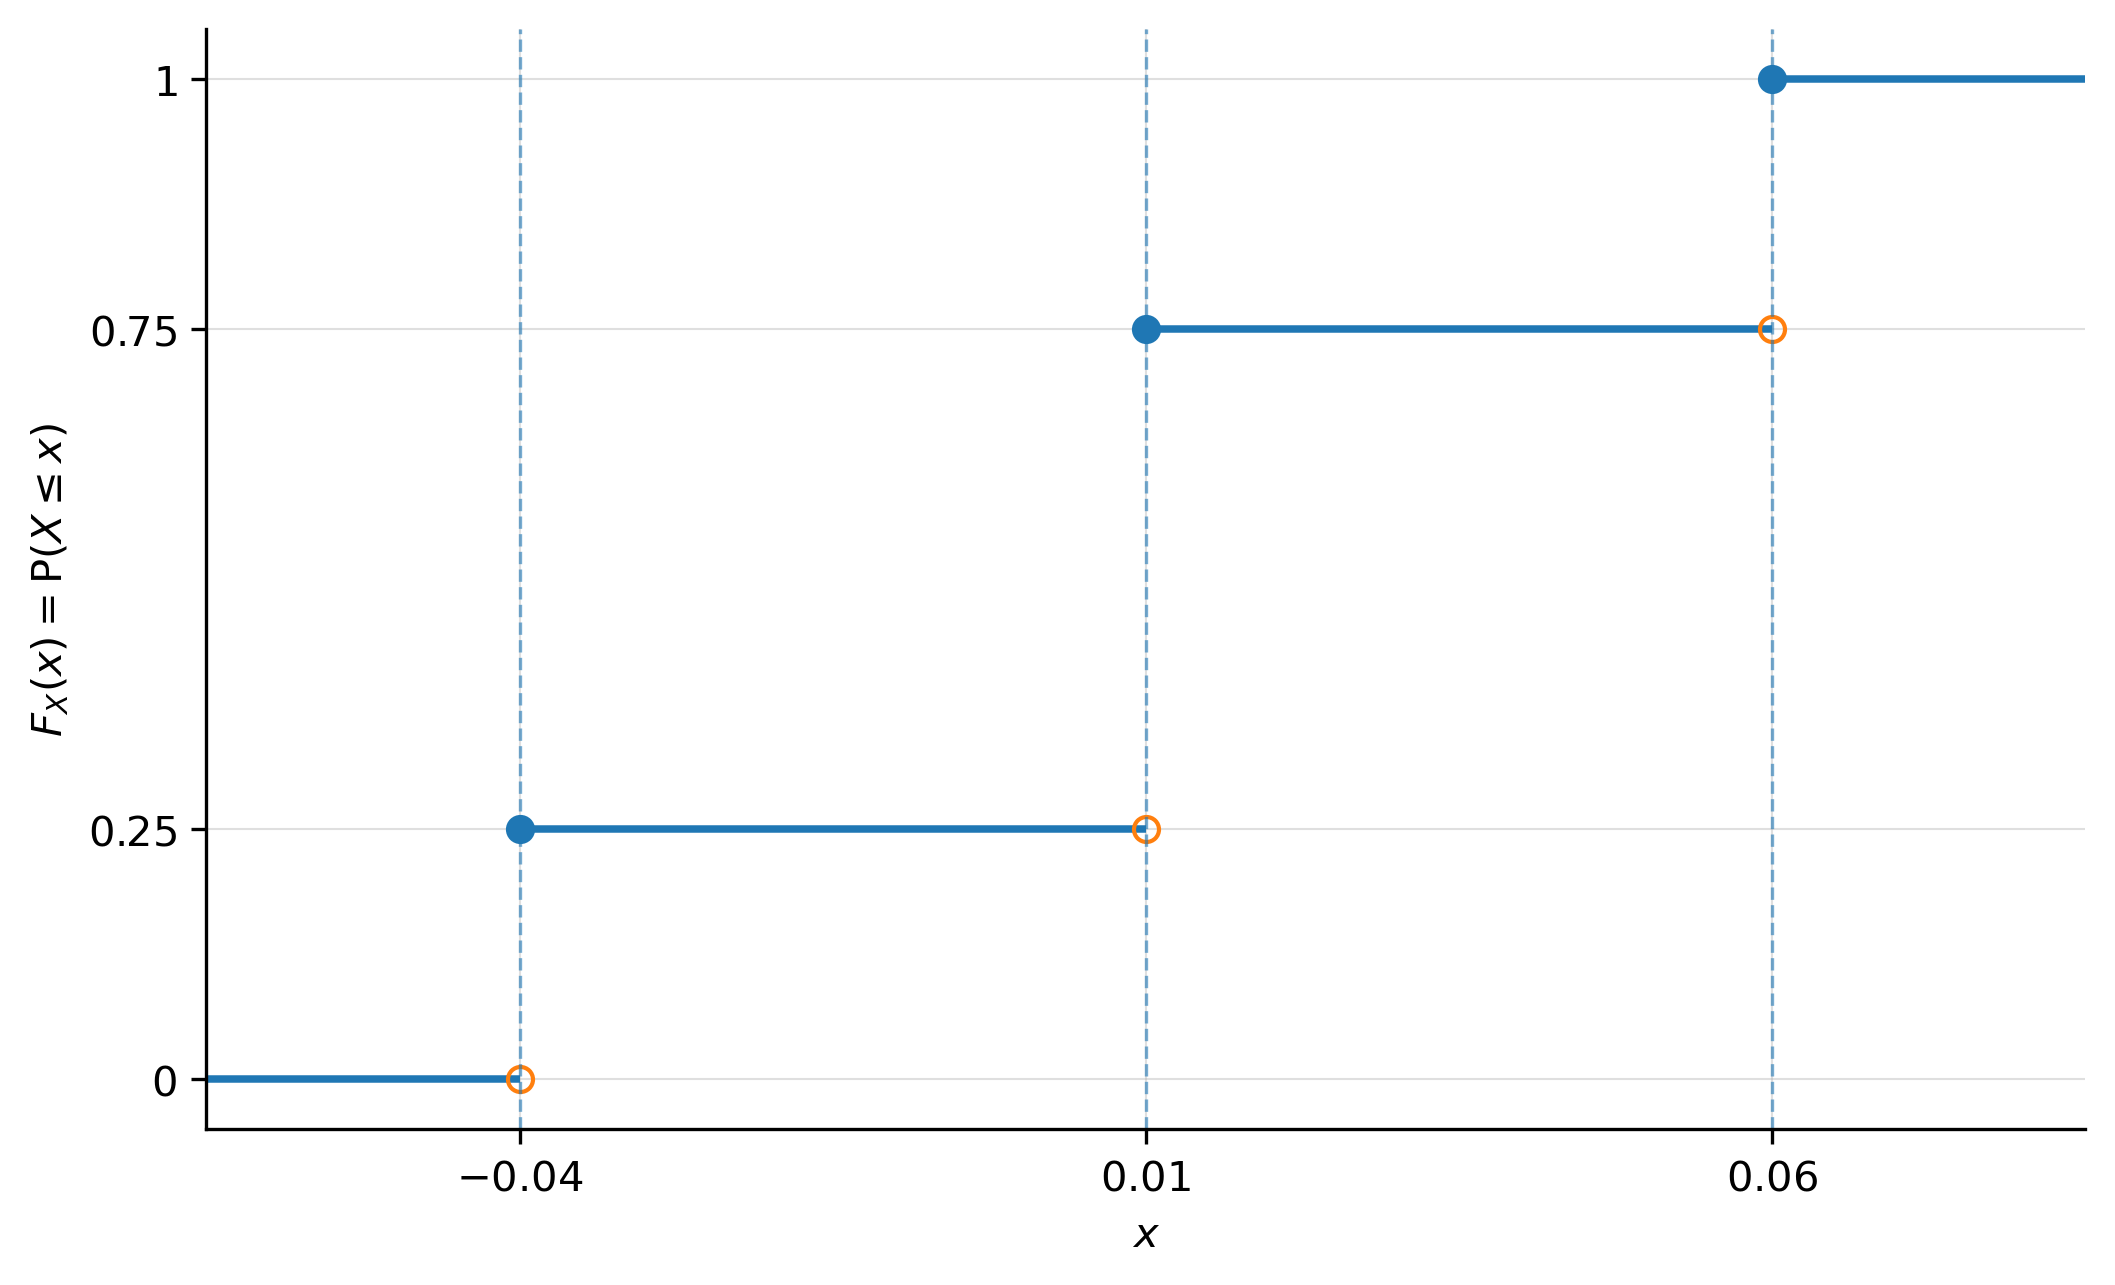
\includegraphics[width=0.78\textwidth]{graphics/cap2_cdf_rendimento_discreto.png}
\end{center}

La continuit\`{a} da destra determina il valore della funzione nei punti di
salto.

%TCIMACRO{\TeXButton{Transition: Box Out}{\transboxout}}%
%BeginExpansion
\transboxout%
%EndExpansion
%TCIMACRO{\TeXButton{EndFrame}{\end{frame}}}%
%BeginExpansion
\end{frame}%
%EndExpansion

%***********************************
\subsection{Variabili casuali continue e densit\`{a}}

%TCIMACRO{\TeXButton{BeginFrame}{\begin{frame}}}%
%BeginExpansion
\begin{frame}%
%EndExpansion

\QTR{frametitle}{Variabili continue e densit\`{a}}

Nel caso continuo, la probabilit\`{a} non \`{e} concentrata sui singoli valori.

\medskip

Una variabile casuale $X$ \`{e} \textbf{assolutamente continua} se esiste una funzione
$f_X:\mathbb{R}\to[0,+\infty)$ tale che

\[
\Prob_X(B)
=
\Prob(X\in B)
=
\int_B f_X(x)\,dx,
\qquad
B\in\mathcal{B}(\mathbb{R}).
\]

\medskip

$f_X$ \`{e} detta \textbf{funzione di densit\`{a}} (di probabilit\`{a}) di $X$.

\medskip

Condizioni fondamentali:

\[
f_X(x)\geq 0,
\qquad
\int_{-\infty}^{+\infty}f_X(x)\,dx=1.
\]

%TCIMACRO{\TeXButton{Transition: Box Out}{\transboxout}}%
%BeginExpansion
\transboxout%
%EndExpansion
%TCIMACRO{\TeXButton{EndFrame}{\end{frame}}}%
%BeginExpansion
\end{frame}%
%EndExpansion

%***********************************
\subsection{Probabilit\`{a} come area}

%TCIMACRO{\TeXButton{BeginFrame}{\begin{frame}}}%
%BeginExpansion
\begin{frame}%
%EndExpansion

\QTR{frametitle}{Probabilit\`{a} come area sotto la densit\`{a}}

Per $a<b$, la probabilit\`{a} che $X$ appartenga all'intervallo $(a,b]$ \`{e}

\[
\Prob(a<X\leq b)
=
\int_a^b f_X(x)\,dx.
\]

\medskip

Nel caso assolutamente continuo, i singoli punti hanno probabilit\`{a} nulla:

\[
\Prob(X=x)=0,
\qquad
x\in\mathbb{R}.
\]

\medskip

Quindi l'inclusione o esclusione degli estremi non modifica la probabilit\`{a}:

\[
\Prob(a<X<b)
=
\Prob(a\leq X\leq b)
=
\int_a^b f_X(x)\,dx.
\]

\medskip

Attenzione: $f_X(x)$ non \`{e} una probabilit\`{a}; la probabilit\`{a} \`{e}
l'area sotto la densit\`{a}.

%TCIMACRO{\TeXButton{Transition: Box Out}{\transboxout}}%
%BeginExpansion
\transboxout%
%EndExpansion
%TCIMACRO{\TeXButton{EndFrame}{\end{frame}}}%
%BeginExpansion
\end{frame}%
%EndExpansion


%***********************************
\subsection{Probabilit\`{a} come area}

%TCIMACRO{\TeXButton{BeginFrame}{\begin{frame}}}%
%BeginExpansion
\begin{frame}%
%EndExpansion

\QTR{frametitle}{Probabilit\`{a} come area sotto la densit\`{a}}

L'area compresa tra $a$ e $b$ rappresenta la probabilit\`{a} che la variabile casuale $X$ assuma valori in quell'intervallo.


\medskip

\begin{center}

\includegraphics[width=0.82\textwidth]{graphics/cap2_probabilita_area_sotto_densita.png}
\end{center}



%TCIMACRO{\TeXButton{Transition: Box Out}{\transboxout}}%
%BeginExpansion
\transboxout%
%EndExpansion
%TCIMACRO{\TeXButton{EndFrame}{\end{frame}}}%
%BeginExpansion
\end{frame}%
%EndExpansion


%***********************************
\subsection{Probabilit\`{a} di un punto}

%TCIMACRO{\TeXButton{BeginFrame}{\begin{frame}}}%
%BeginExpansion
\begin{frame}%
%EndExpansion

\QTR{frametitle}{Se l'intervallo si restringe a un punto}

Se l'intervallo $[a,b]$ si restringe, l'area sottesa dalla densit\`{a} tende a
zero.

\[
a\leftarrow b
\qquad\Longrightarrow\qquad
\int_a^a f_X(x)\,dx\to 0
\]

\medskip

Quindi, nel caso assolutamente continuo,

\[
\Prob(X=a)=0.
\]

\medskip

Pi\`{u} in generale,

\[
\Prob(X=x)=0,
\qquad
x\in\mathbb{R}.
\]

\medskip

La probabilit\`{a} non \`{e} attribuita ai singoli punti, ma agli intervalli,
cio\`{e} alle aree sotto la densit\`{a}.

%TCIMACRO{\TeXButton{Transition: Box Out}{\transboxout}}%
%BeginExpansion
\transboxout%
%EndExpansion
%TCIMACRO{\TeXButton{EndFrame}{\end{frame}}}%
%BeginExpansion
\end{frame}%
%EndExpansion


%***********************************
\subsection{Densit\`{a} e funzione di distribuzione}

%TCIMACRO{\TeXButton{BeginFrame}{\begin{frame}}}%
%BeginExpansion
\begin{frame}%
%EndExpansion

\QTR{frametitle}{Densit\`{a} e funzione di distribuzione}

La funzione di distribuzione si ottiene integrando la densit\`{a}:

\[
F_X(x)
=
\Prob(X\leq x)
=
\int_{-\infty}^{x} f_X(s)\,ds.
\]

\medskip

Se $F_X$ \`{e} derivabile nel punto $x$, allora

\[
f_X(x)=F_X'(x).
\]

\medskip

Interpretazione locale:

\[
\Prob\left(x-\frac{\varepsilon}{2}<X\leq x+\frac{\varepsilon}{2}\right)
\simeq
\varepsilon f_X(x),
\qquad
\varepsilon \mbox{ piccolo}.
\]

\medskip

La densit\`{a} misura la rapidit\`{a} con cui la probabilit\`{a} si accumula
intorno a un valore.

%TCIMACRO{\TeXButton{Transition: Box Out}{\transboxout}}%
%BeginExpansion
\transboxout%
%EndExpansion
%TCIMACRO{\TeXButton{EndFrame}{\end{frame}}}%
%BeginExpansion
\end{frame}%
%EndExpansion


%***********************************
\subsection{Esempio uniforme}

%TCIMACRO{\TeXButton{BeginFrame}{\begin{frame}}}%
%BeginExpansion
\begin{frame}%
%EndExpansion

\QTR{frametitle}{Esempio: rendimento uniforme}

Sia $R$ un rendimento continuo con densit\`{a} uniforme su $[-0.04,0.06]$:

\[
f_R(r)=
\begin{cases}
10, & -0.04\leq r\leq 0.06,\\
0, & \mbox{altrove}.
\end{cases}
\]

\medskip

La densit\`{a} \`{e} costante sull'intervallo dei valori possibili.

\[
\int_{-\infty}^{+\infty} f_R(r)\,dr
=
\int_{-0.04}^{0.06}10\,dr
=
10(0.10)
=
1.
\]

\medskip

La normalizzazione conferma che $f_R$ \`{e} una densit\`{a} di probabilit\`{a}.

%TCIMACRO{\TeXButton{Transition: Box Out}{\transboxout}}%
%BeginExpansion
\transboxout%
%EndExpansion
%TCIMACRO{\TeXButton{EndFrame}{\end{frame}}}%
%BeginExpansion
\end{frame}%
%EndExpansion


%***********************************
\subsection{Area di probabilit\`{a} nell'esempio uniforme}

%TCIMACRO{\TeXButton{BeginFrame}{\begin{frame}}}%
%BeginExpansion
\begin{frame}%
%EndExpansion

\QTR{frametitle}{Esempio uniforme: probabilit\`{a} di un intervallo}

L'area evidenziata rappresenta la probabilit\`{a} che il rendimento sia compreso
tra $1\%$ e $5\%$.

\medskip

\begin{center}
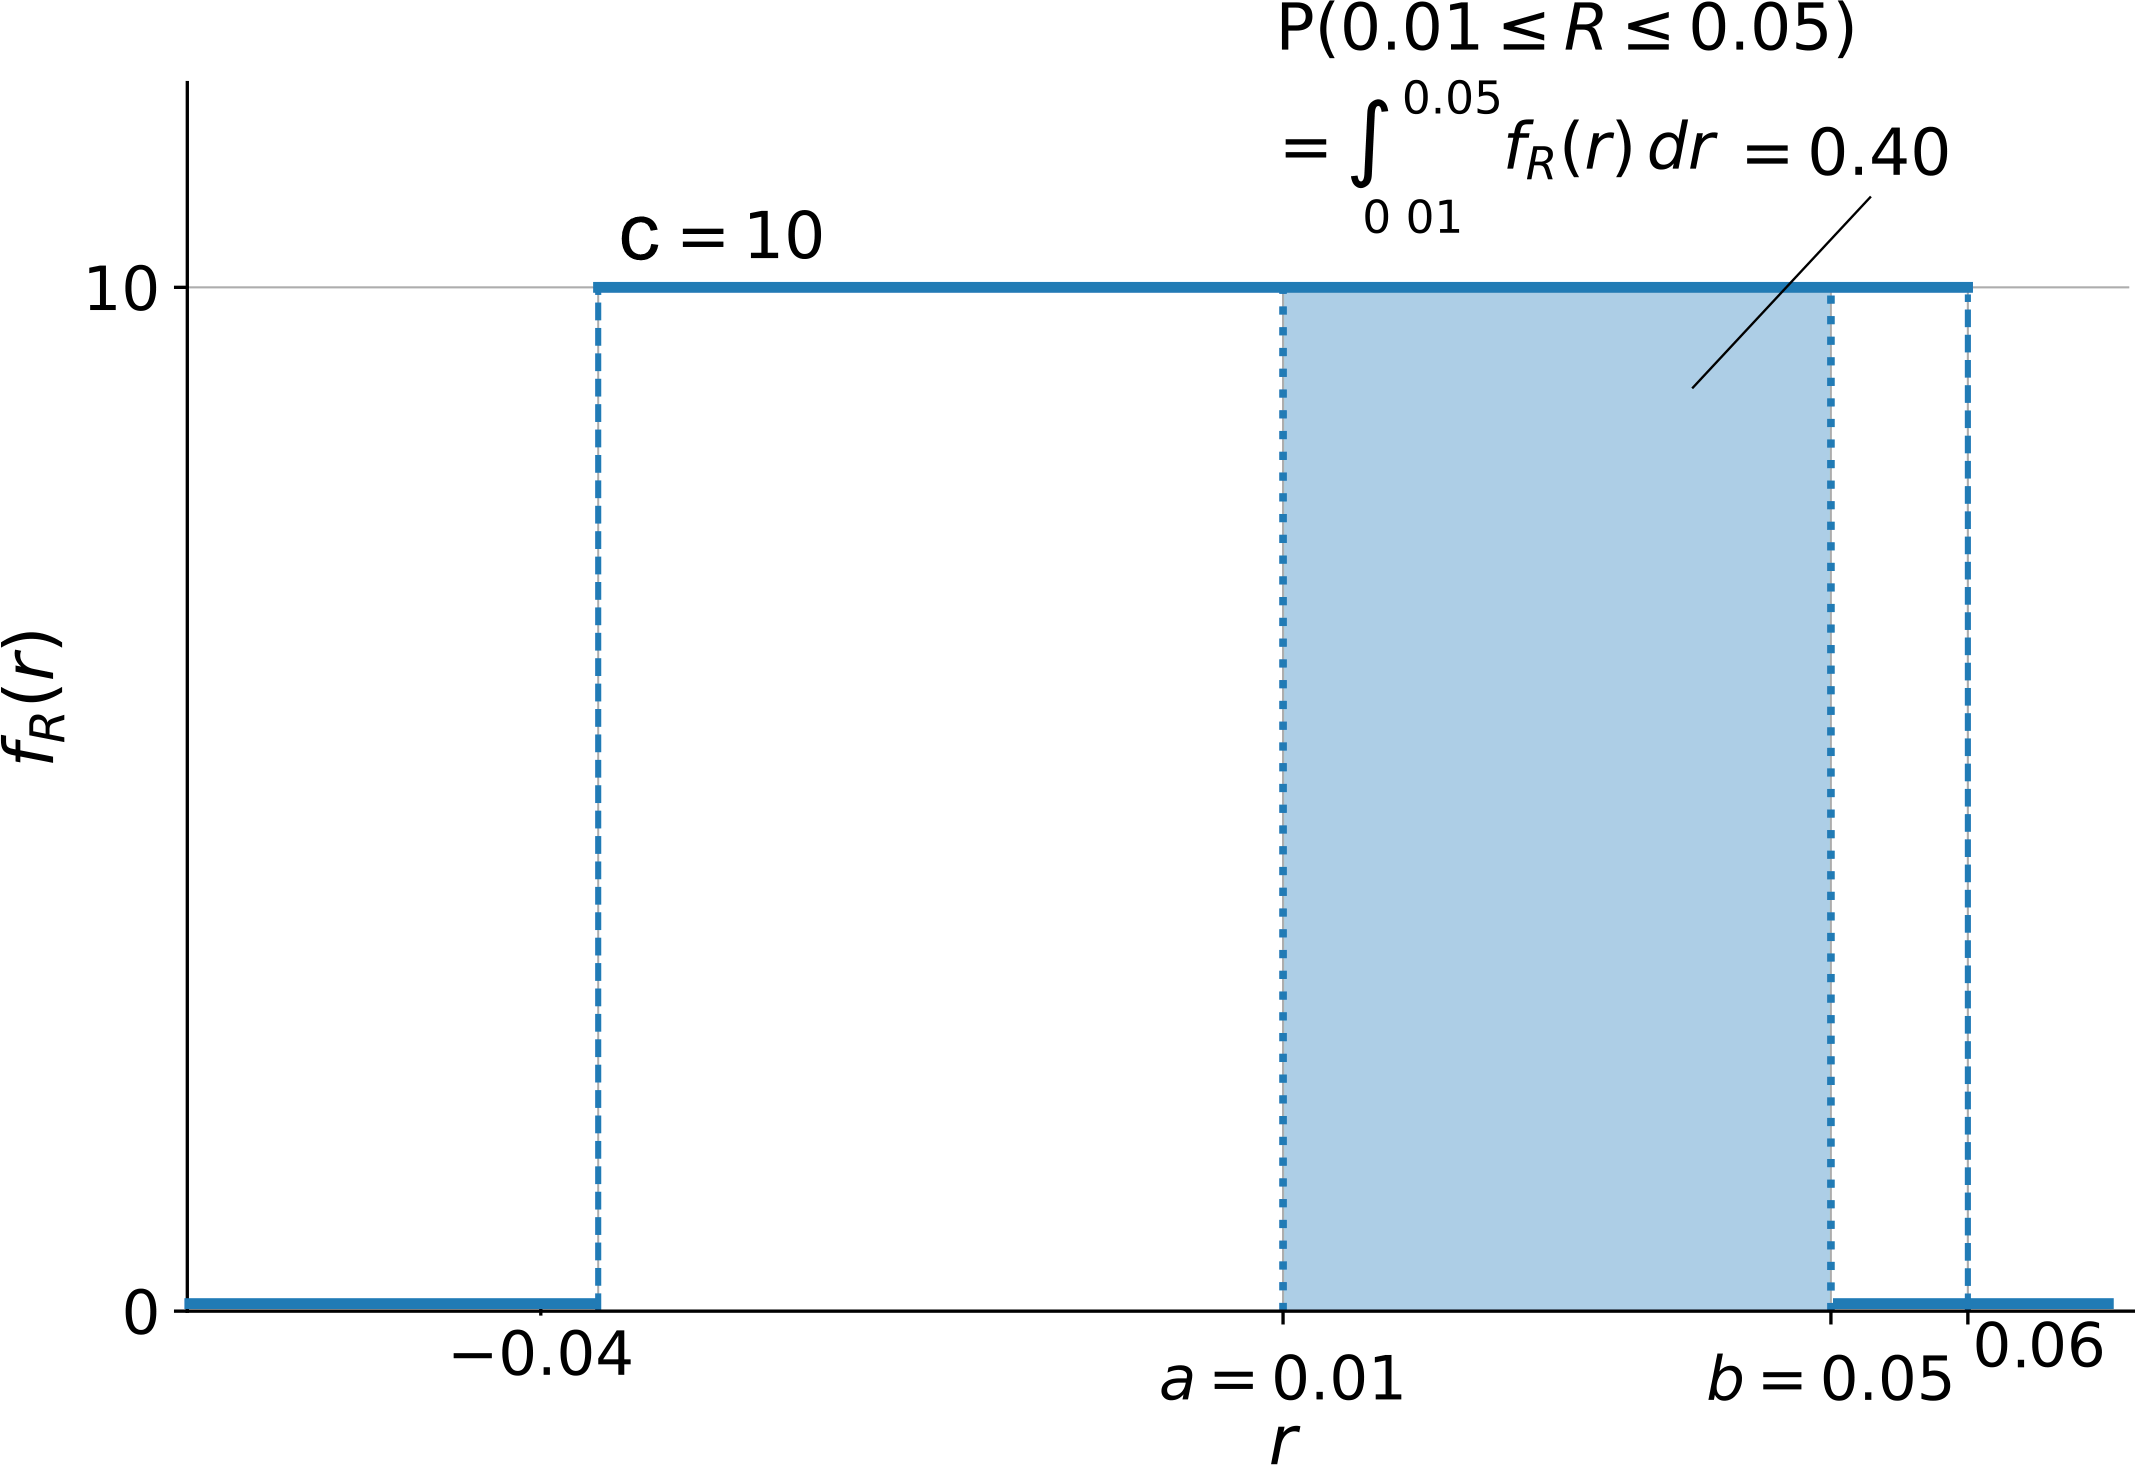
\includegraphics[width=0.78\textwidth]{graphics/cap2_densita_uniforme_rendimento_area_01_05.png}
\end{center}

%TCIMACRO{\TeXButton{Transition: Box Out}{\transboxout}}%
%BeginExpansion
\transboxout%
%EndExpansion
%TCIMACRO{\TeXButton{EndFrame}{\end{frame}}}%
%BeginExpansion
\end{frame}%
%EndExpansion

%***********************************
\subsection{Probabilit\`{a} di coda}

%TCIMACRO{\TeXButton{BeginFrame}{\begin{frame}}}%
%BeginExpansion
\begin{frame}%
%EndExpansion

\QTR{frametitle}{Probabilit\`{a} di coda}

La funzione di distribuzione descrive direttamente le probabilit\`{a} di coda.

\medskip

Coda sinistra:

\[
\Prob(X\leq x)=F_X(x).
\]

\medskip

Coda destra:

\[
\Prob(X>x)=1-F_X(x).
\]

\medskip

Per eventi con disuguaglianza non stretta:

\[
\Prob(X\geq x)=1-F_X(x^-).
\]

\medskip

Se $L$ rappresenta una perdita, la probabilit\`{a}

\[
\Prob(L>\ell)
\]

misura la probabilit\`{a} che la perdita superi la soglia $\ell$.

%TCIMACRO{\TeXButton{Transition: Box Out}{\transboxout}}%
%BeginExpansion
\transboxout%
%EndExpansion
%TCIMACRO{\TeXButton{EndFrame}{\end{frame}}}%
%BeginExpansion
\end{frame}%
%EndExpansion


%***********************************
\subsection{Quantili}

%TCIMACRO{\TeXButton{BeginFrame}{\begin{frame}}}%
%BeginExpansion
\begin{frame}%
%EndExpansion

\QTR{frametitle}{Quantile di ordine $\alpha$}

Sia $X$ una variabile casuale reale con funzione di distribuzione $F_X$.

\medskip

Per $\alpha\in(0,1)$, il quantile di ordine $\alpha$ \`{e}

\[
q_\alpha(X)
=
\inf\{x\in\mathbb{R}:F_X(x)\geq \alpha\}.
\]

\medskip

Il quantile \`{e} la soglia pi\`{u} bassa per cui la probabilit\`{a} cumulata
raggiunge almeno $\alpha$.

\medskip

La definizione tramite infimo \`{e} valida anche quando $F_X$ presenta salti.

\medskip

Nel caso discreto, il quantile pu\`{o} coincidere con un punto di salto della
funzione di distribuzione.

%TCIMACRO{\TeXButton{Transition: Box Out}{\transboxout}}%
%BeginExpansion
\transboxout%
%EndExpansion
%TCIMACRO{\TeXButton{EndFrame}{\end{frame}}}%
%BeginExpansion
\end{frame}%
%EndExpansion


%***********************************
\subsection{Quantili nel caso continuo}

%TCIMACRO{\TeXButton{BeginFrame}{\begin{frame}}}%
%BeginExpansion
\begin{frame}%
%EndExpansion

\QTR{frametitle}{Quantili nel caso continuo}

Se $X$ \`{e} assolutamente continua e $F_X$ \`{e} continua e strettamente
crescente nell'intervallo rilevante, il quantile si ottiene risolvendo

\[
F_X(x)=\alpha.
\]

\medskip

In questo caso,

\[
q_\alpha(X)=F_X^{-1}(\alpha).
\]

\medskip

Equivalentemente, se $X$ ha densit\`{a} $f_X$,

\[
\int_{-\infty}^{q_\alpha(X)} f_X(x)\,dx=\alpha.
\]

\medskip

Il quantile individua il punto che lascia a sinistra una probabilit\`{a} pari ad
$\alpha$.

%TCIMACRO{\TeXButton{Transition: Box Out}{\transboxout}}%
%BeginExpansion
\transboxout%
%EndExpansion
%TCIMACRO{\TeXButton{EndFrame}{\end{frame}}}%
%BeginExpansion
\end{frame}%
%EndExpansion


%***********************************
\subsection{Quantile e rischio di perdita}

%TCIMACRO{\TeXButton{BeginFrame}{\begin{frame}}}%
%BeginExpansion
\begin{frame}%
%EndExpansion

\QTR{frametitle}{Quantile e rischio di perdita}

Se $L$ rappresenta una perdita, un quantile elevato individua una \textbf{soglia di
rischio}.

\medskip

Per $\alpha$ vicino a $1$,

\[
q_\alpha(L)
\]

\`{e} una soglia tale che la perdita resta sotto quel livello con probabilit\`{a}
almeno $\alpha$. Nel \textbf{caso continuo},

\[
\Prob(L\leq q_\alpha(L))=\alpha,
\]

\medskip

e quindi, perdite di importo maggiore a $q_\alpha(L)$ avranno probabilità:
\[
\Prob(L>q_\alpha(L))=1-\alpha.
\]

\medskip

Esempio: $q_{0.99}(L)$ \`{e} una soglia superata solo con
probabilit\`{a} pari all'$1\%$.

%TCIMACRO{\TeXButton{Transition: Box Out}{\transboxout}}%
%BeginExpansion
\transboxout%
%EndExpansion
%TCIMACRO{\TeXButton{EndFrame}{\end{frame}}}%
%BeginExpansion
\end{frame}%
%EndExpansion


%***********************************
\subsection{Quantile normale: esempio}

%TCIMACRO{\TeXButton{BeginFrame}{\begin{frame}}}%
%BeginExpansion
\begin{frame}%
%EndExpansion

\QTR{frametitle}{Coda sinistra e quantile: esempio normale}

Consideriamo un rendimento normale:

\[
R\sim\mathcal{N}(0.008,0.035^2).
\]

\medskip

Il quantile al $5\%$ si ottiene da

\[
q_{0.05}(R)=\mu+\sigma z_{0.05},
\]

dove

\[
z_{0.05}\simeq -1.645.
\]

\medskip

Quindi

\[
q_{0.05}(R)
=
0.008+0.035(-1.645)
\simeq
-0.0496.
\]

\medskip

Interpretazione: il $5\%$ peggiore dei rendimenti si colloca al di sotto di
circa $-4.96\%$.

%TCIMACRO{\TeXButton{Transition: Box Out}{\transboxout}}%
%BeginExpansion
\transboxout%
%EndExpansion
%TCIMACRO{\TeXButton{EndFrame}{\end{frame}}}%
%BeginExpansion
\end{frame}%
%EndExpansion


%***********************************
\subsection{Quantile normale: grafico}

%TCIMACRO{\TeXButton{BeginFrame}{\begin{frame}}}%
%BeginExpansion
\begin{frame}%
%EndExpansion

\QTR{frametitle}{Coda sinistra e quantile: rappresentazione grafica}

\begin{center}
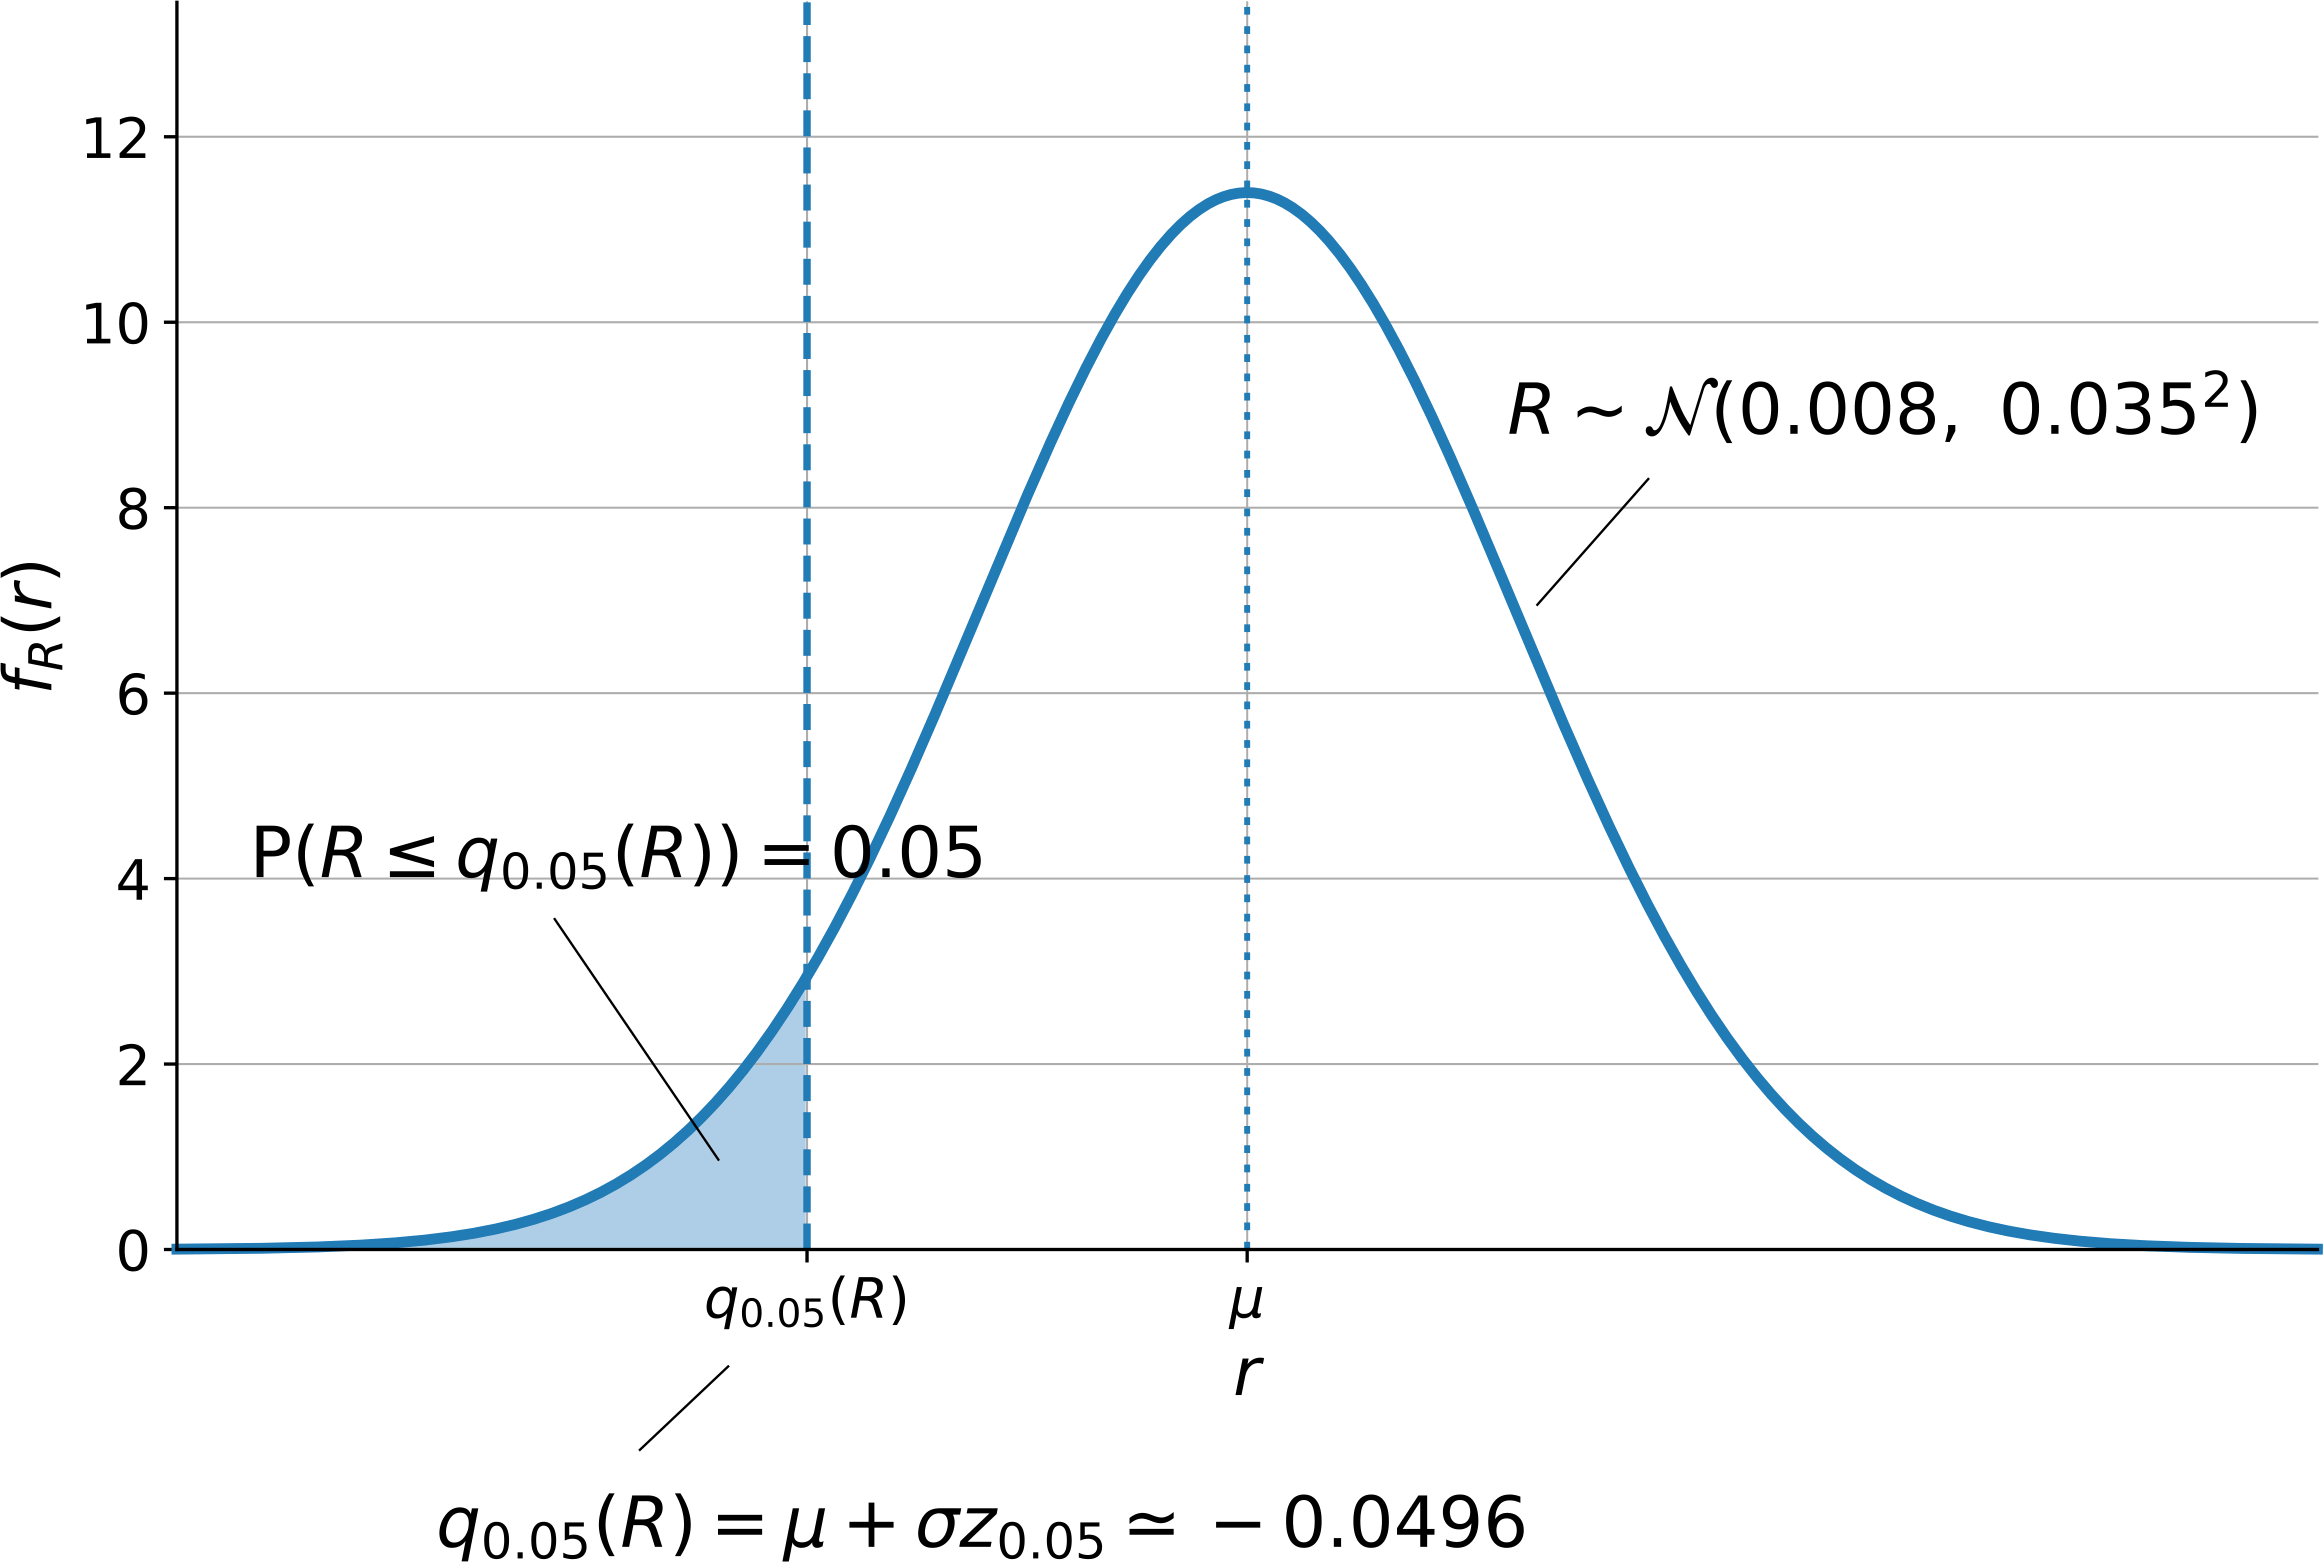
\includegraphics[width=0.80\textwidth]{graphics/cap2_normale_coda_sinistra_quantile_05.png}
\end{center}

%TCIMACRO{\TeXButton{Transition: Box Out}{\transboxout}}%
%BeginExpansion
\transboxout%
%EndExpansion
%TCIMACRO{\TeXButton{EndFrame}{\end{frame}}}%
%BeginExpansion
\end{frame}%
%EndExpansion

%***********************************
\subsection{Valore atteso}

%TCIMACRO{\TeXButton{BeginFrame}{\begin{frame}}}%
%BeginExpansion
\begin{frame}%
%EndExpansion

\QTR{frametitle}{Valore atteso}

Il valore atteso sintetizza la posizione media della distribuzione.

\medskip

Caso discreto:

\[
\E[X]
=
\sum_i x_i p_X(x_i).
\]

\medskip

Caso assolutamente continuo:

\[
\E[X]
=
\int_{-\infty}^{+\infty}x f_X(x)\,dx.
\]

\medskip

Interpretazione finanziaria:

\[
\begin{array}{rcl}
\E[R] & : & \mbox{rendimento medio atteso},\\[4pt]
\E[L] & : & \mbox{perdita attesa},\\[4pt]
\E[H] & : & \mbox{payoff medio}.
\end{array}
\]

\medskip

Il valore atteso \`{e} una media probabilistica, non una previsione deterministica.

%TCIMACRO{\TeXButton{Transition: Box Out}{\transboxout}}%
%BeginExpansion
\transboxout%
%EndExpansion
%TCIMACRO{\TeXButton{EndFrame}{\end{frame}}}%
%BeginExpansion
\end{frame}%
%EndExpansion


%***********************************
\subsection{Linearit\`{a} del valore atteso}

%TCIMACRO{\TeXButton{BeginFrame}{\begin{frame}}}%
%BeginExpansion
\begin{frame}%
%EndExpansion

\QTR{frametitle}{Linearit\`{a} del valore atteso}

Se $a$ e $b$ sono costanti reali, allora

\[
\E[aX+b]
=
a\E[X]+b.
\]

\medskip

Pi\`{u} in generale,

\[
\E\left[\sum_{i=1}^n a_iX_i\right]
=
\sum_{i=1}^n a_i\E[X_i].
\]

\medskip

Questa propriet\`{a} non richiede indipendenza tra le variabili casuali.

\medskip

Applicazione finanziaria:

\[
R_P=\sum_{i=1}^n w_i R_i
\qquad\Longrightarrow\qquad
\E[R_P]=\sum_{i=1}^n w_i\E[R_i].
\]

\medskip

La linearit\`{a} \`{e} essenziale per rendimenti di portafoglio e trasformazioni
affini.

%TCIMACRO{\TeXButton{Transition: Box Out}{\transboxout}}%
%BeginExpansion
\transboxout%
%EndExpansion
%TCIMACRO{\TeXButton{EndFrame}{\end{frame}}}%
%BeginExpansion
\end{frame}%
%EndExpansion


%***********************************
\subsection{Valore atteso di funzioni}

%TCIMACRO{\TeXButton{BeginFrame}{\begin{frame}}}%
%BeginExpansion
\begin{frame}%
%EndExpansion

\QTR{frametitle}{Valore atteso di $g(X)$}

Spesso l'oggetto finanziario rilevante non \`{e} $X$, ma una funzione di $X$.

\[
Y=g(X).
\]

\medskip

Caso discreto:

\[
\E[g(X)]
=
\sum_i g(x_i)p_X(x_i).
\]

\medskip

Caso assolutamente continuo:

\[
\E[g(X)]
=
\int_{-\infty}^{+\infty} g(x)f_X(x)\,dx.
\]

%TCIMACRO{\TeXButton{Transition: Box Out}{\transboxout}}%
%BeginExpansion
\transboxout%
%EndExpansion
%TCIMACRO{\TeXButton{EndFrame}{\end{frame}}}%
%BeginExpansion
\end{frame}%
%EndExpansion


%***********************************

%TCIMACRO{\TeXButton{BeginFrame}{\begin{frame}}}%
%BeginExpansion
\begin{frame}%
%EndExpansion

\QTR{frametitle}{Valore atteso di $g(X)$}

Esempio: payoff di una call europea

\[
H=(S_T-K)^+.
\]

\[
\E[H]
=
\E[(S_T-K)^+].
\]

\medskip

In generale,

\[
\E[g(X)]\neq g(\E[X])
\]

quando $g$ non \`{e} lineare.

%TCIMACRO{\TeXButton{Transition: Box Out}{\transboxout}}%
%BeginExpansion
\transboxout%
%EndExpansion
%TCIMACRO{\TeXButton{EndFrame}{\end{frame}}}%
%BeginExpansion
\end{frame}%
%EndExpansion


%***********************************
\subsection{Variabili indicatrici}

%TCIMACRO{\TeXButton{BeginFrame}{\begin{frame}}}%
%BeginExpansion
\begin{frame}%
%EndExpansion

\QTR{frametitle}{Variabili indicatrici}

Il valore atteso di una variabile indicatrice coincide con la probabilit\`{a}
dell'evento corrispondente:

\[
\E[\mathbf{1}_A]
=
\Prob(A).
\]

\medskip

Esempi finanziari:

\[
\E[\mathbf{1}_{\{R<0\}}]
=
\Prob(R<0),
\]

\[
\E[\mathbf{1}_{\{L>\ell\}}]
=
\Prob(L>\ell),
\]

\[
\E[\mathbf{1}_{\{S_T>K\}}]
=
\Prob(S_T>K).
\]

\medskip

Le variabili indicatrici trasformano eventi in variabili casuali a valori
$0$ e $1$.

%TCIMACRO{\TeXButton{Transition: Box Out}{\transboxout}}%
%BeginExpansion
\transboxout%
%EndExpansion
%TCIMACRO{\TeXButton{EndFrame}{\end{frame}}}%
%BeginExpansion
\end{frame}%
%EndExpansion



%***********************************
\subsection{Indicatrice dell'evento di rendimento negativo}

%TCIMACRO{\TeXButton{BeginFrame}{\begin{frame}}}%
%BeginExpansion
\begin{frame}%
%EndExpansion

\QTR{frametitle}{Indicatrice dell'evento di rendimento negativo}

Sia $r$ uno dei possibili valori della variabile casuale $R$, rendimento di un portafoglio.

\medskip

La funzione indicatrice indicatrice dell'evento "rendimento negativo" \`{e}:

\[
\mathbf{1}_{\{R<0\}}=
\begin{cases}
1, & \mbox{se } R<0,\\
0, & \mbox{se } R\geq 0.
\end{cases}
\]

\medskip

Il suo valore atteso ha una chiara interpretazione:

\medskip

\[
\E[\mathbf{1}_{\{R<0\}}]
=
\Prob(R<0).
\]

%TCIMACRO{\TeXButton{Transition: Box Out}{\transboxout}}%
%BeginExpansion
\transboxout%
%EndExpansion
%TCIMACRO{\TeXButton{EndFrame}{\end{frame}}}%
%BeginExpansion
\end{frame}%
%EndExpansion


%***********************************
\subsection{Shortfall}

%TCIMACRO{\TeXButton{BeginFrame}{\begin{frame}}}%
%BeginExpansion
\begin{frame}%
%EndExpansion

\QTR{frametitle}{Perdita percentuale rispetto alla soglia zero: grafico}

Introduciamo la funzione $g(r)$, perdita percentuale:

\[
g(r)=(-r)^+=-r\,\mathbf{1}_{\{r<0\}}.
\]

\medskip

\begin{center}
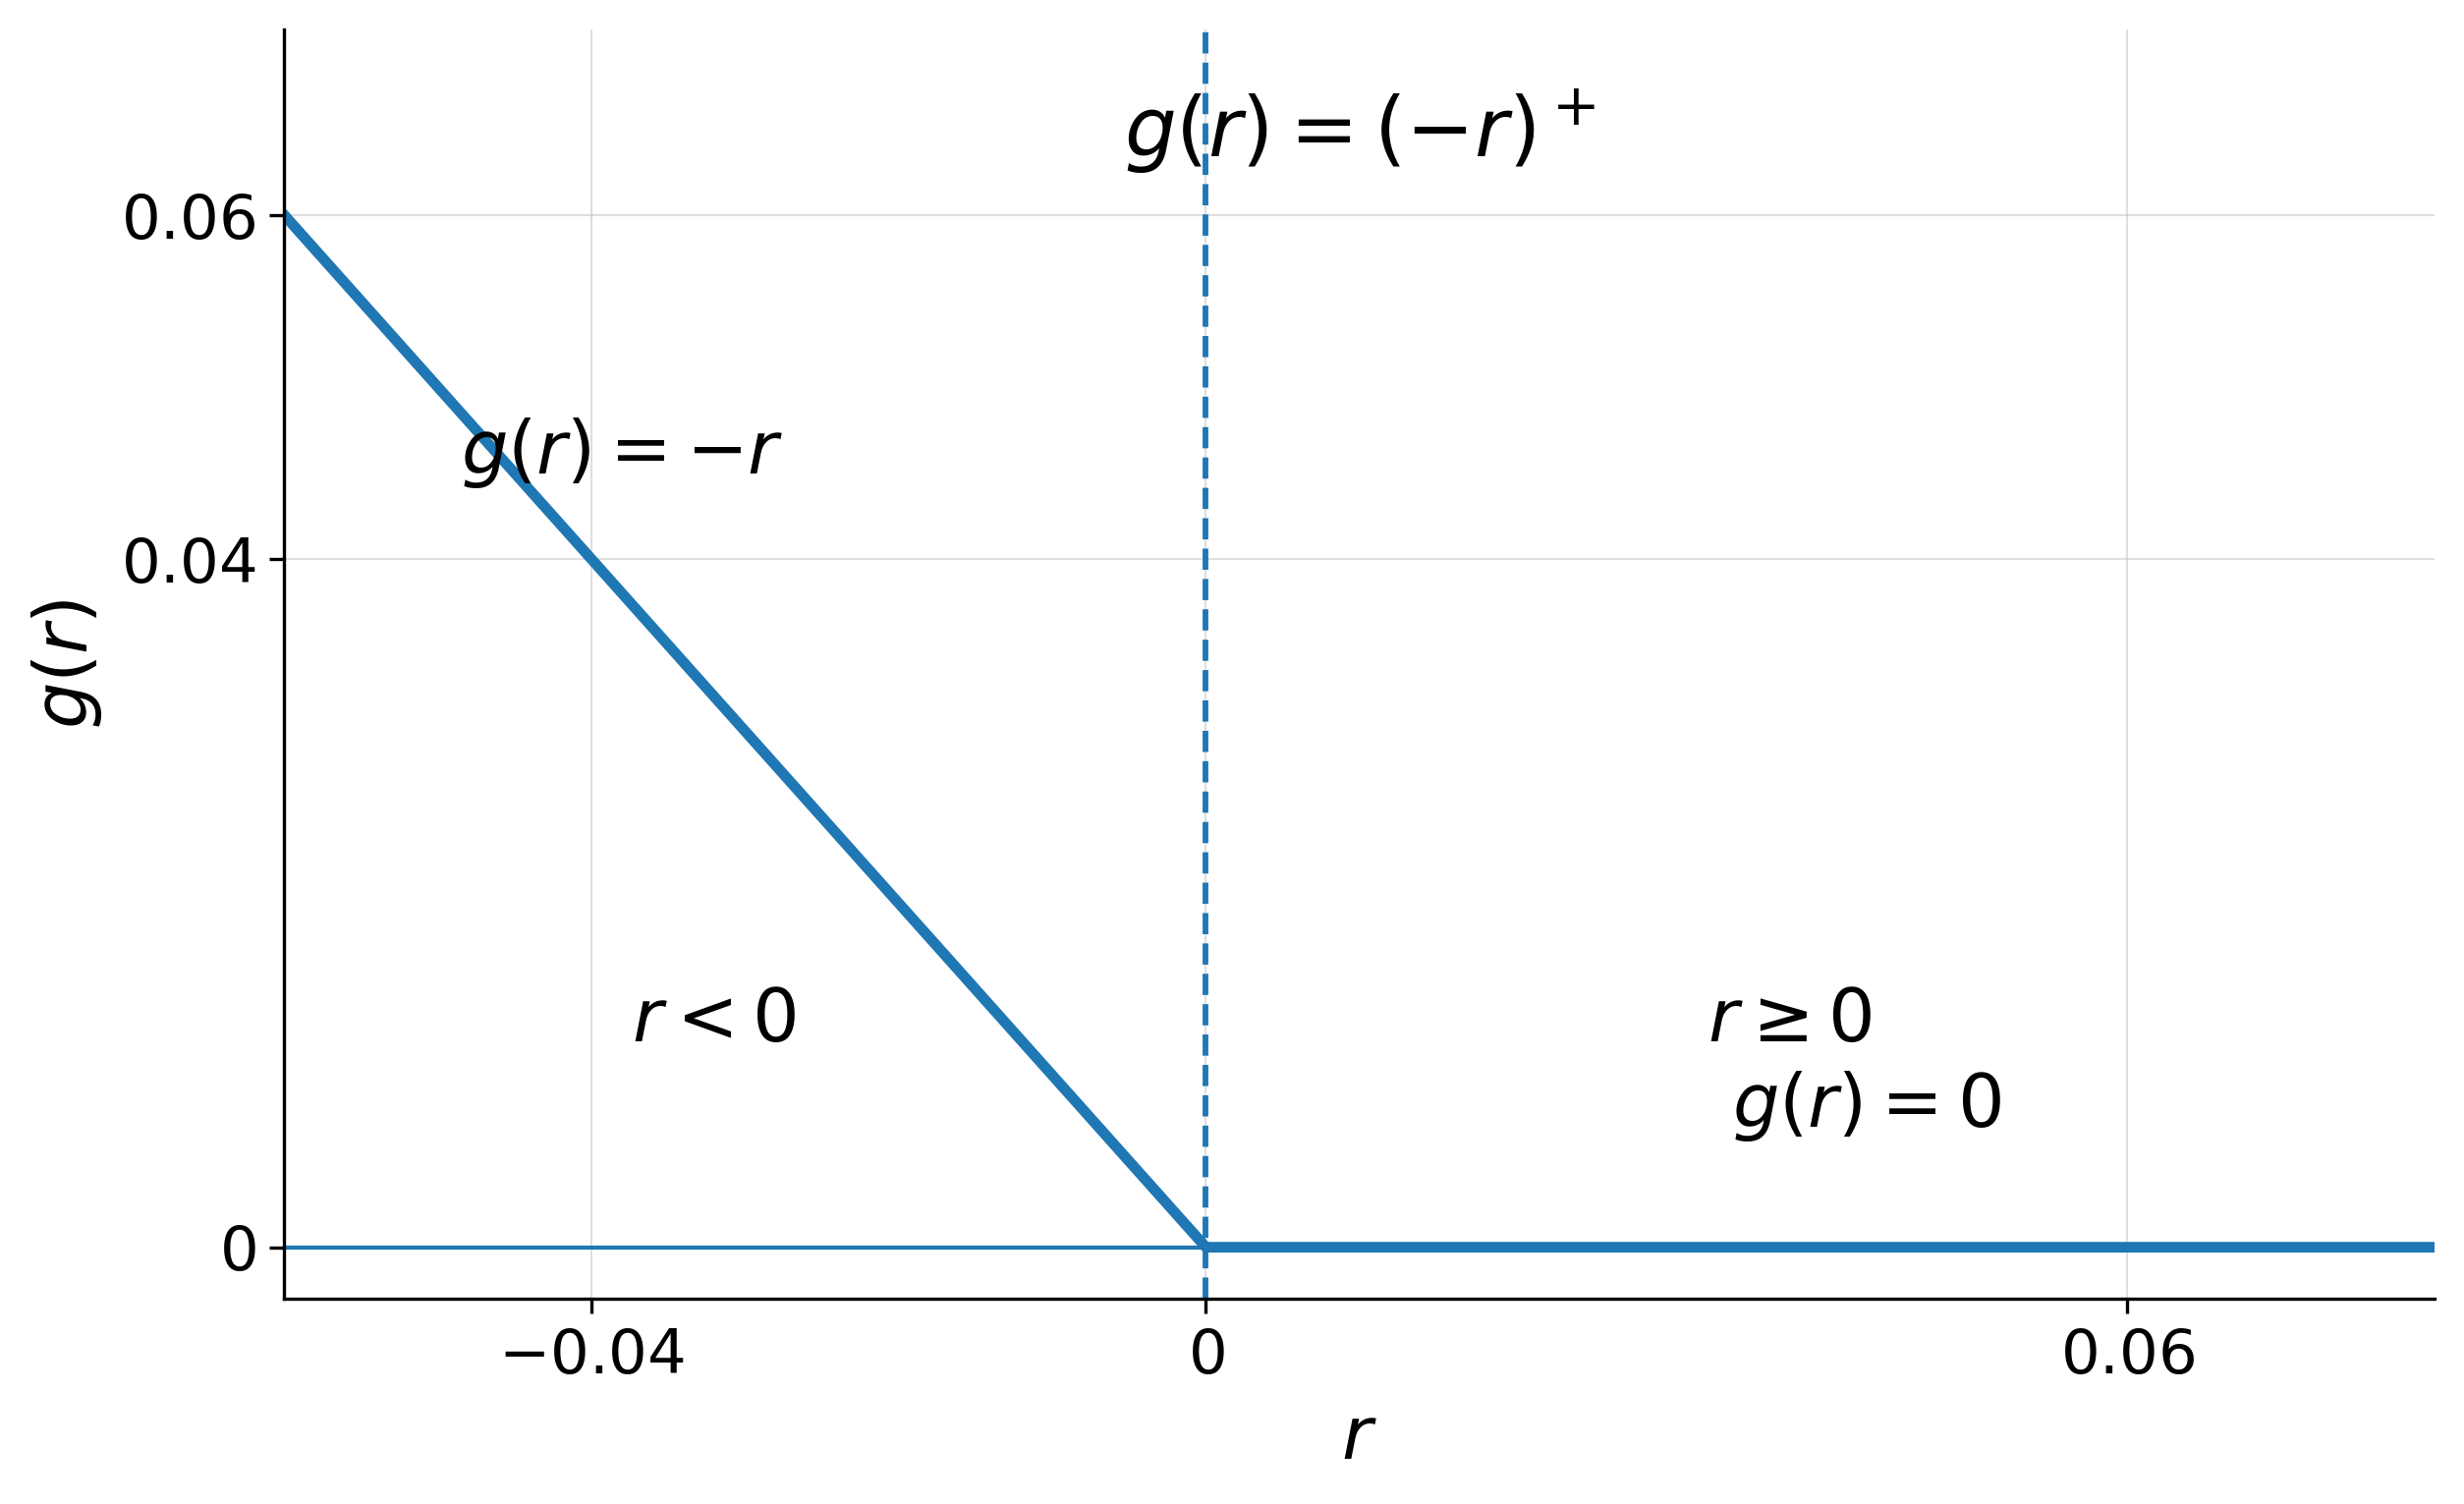
\includegraphics[width=0.80\textwidth]{graphics/cap2_funzione_shortfall_zero.png}
\end{center}

%TCIMACRO{\TeXButton{Transition: Box Out}{\transboxout}}%
%BeginExpansion
\transboxout%
%EndExpansion
%TCIMACRO{\TeXButton{EndFrame}{\end{frame}}}%
%BeginExpansion
\end{frame}%
%EndExpansion


%***********************************

%TCIMACRO{\TeXButton{BeginFrame}{\begin{frame}}}%
%BeginExpansion
\begin{frame}%
%EndExpansion

\QTR{frametitle}{Shortfall come valore atteso condizionato}


Un indicatore di interesse finanziario è lo \emph{shortfall}, inteso come valore atteso della perdita condizionato al verificarsi di un rendimento negativo:

\[
\operatorname{SF}
=
\mathbb{E}[g(r)\mid r<0]
=
\mathbb{E}[-r\mid r<0].
\]

Esso rappresenta quindi la perdita percentuale media osservata nei soli scenari sfavorevoli.

%TCIMACRO{\TeXButton{Transition: Box Out}{\transboxout}}%
%BeginExpansion
\transboxout%
%EndExpansion
%TCIMACRO{\TeXButton{EndFrame}{\end{frame}}}%
%BeginExpansion
\end{frame}%
%EndExpansion

%***********************************
\subsection{Varianza}

%TCIMACRO{\TeXButton{BeginFrame}{\begin{frame}}}%
%BeginExpansion
\begin{frame}%
%EndExpansion

\QTR{frametitle}{Varianza: dispersione intorno alla media}

Il valore atteso descrive la posizione media della distribuzione, ma non misura
la dispersione.

\medskip

La varianza di $X$ \`{e}

\[
\Var(X)
=
\E\left[(X-\E[X])^2\right].
\]

\medskip

Nel caso discreto,

\[
\Var(X)
=
\sum_i (x_i-\E[X])^2p_X(x_i).
\]

\medskip

Nel caso assolutamente continuo,

\[
\Var(X)
=
\int_{-\infty}^{+\infty}(x-\E[X])^2f_X(x)\,dx.
\]

\medskip

La varianza misura lo scostamento quadratico medio dal valore atteso.

%TCIMACRO{\TeXButton{Transition: Box Out}{\transboxout}}%
%BeginExpansion
\transboxout%
%EndExpansion
%TCIMACRO{\TeXButton{EndFrame}{\end{frame}}}%
%BeginExpansion
\end{frame}%
%EndExpansion


%***********************************
\subsection{Formula operativa e deviazione standard}

%TCIMACRO{\TeXButton{BeginFrame}{\begin{frame}}}%
%BeginExpansion
\begin{frame}%
%EndExpansion

\QTR{frametitle}{Formula operativa e deviazione standard}

Una formula utile nei calcoli \`{e}

\[
\Var(X)
=
\E[X^2]-(\E[X])^2.
\]

\medskip

La deviazione standard \`{e}

\[
\sigma_X
=
\sqrt{\Var(X)}.
\]

\medskip

\[
\begin{array}{rcl}
\Var(X) & : & \mbox{dispersione quadratica},\\[4pt]
\sigma_X & : & \mbox{dispersione nella stessa unit\`{a} di } X.
\end{array}
\]

\medskip

Se $a$ e $b$ sono costanti reali,

\[
\Var(aX+b)=a^2\Var(X),
\]

\[
\sigma_{aX+b}=|a|\sigma_X.
\]

\medskip

La traslazione cambia il livello; la scala cambia la dispersione.

%TCIMACRO{\TeXButton{Transition: Box Out}{\transboxout}}%
%BeginExpansion
\transboxout%
%EndExpansion
%TCIMACRO{\TeXButton{EndFrame}{\end{frame}}}%
%BeginExpansion
\end{frame}%
%EndExpansion


%***********************************
\subsection{Momenti centrali}

%TCIMACRO{\TeXButton{BeginFrame}{\begin{frame}}}%
%BeginExpansion
\begin{frame}%
%EndExpansion

\QTR{frametitle}{Momenti centrali e forma della distribuzione}

I momenti centrali descrivono caratteristiche della distribuzione intorno alla
media.

\[
\E[(X-\E[X])^m].
\]

\medskip

Casi principali:

\[
\begin{array}{rcl}
m=2 & : & \Var(X),\\[4pt]
m=3 & : & \mbox{asimmetria},\\[4pt]
m=4 & : & \mbox{peso delle code}.
\end{array}
\]

%TCIMACRO{\TeXButton{Transition: Box Out}{\transboxout}}%
%BeginExpansion
\transboxout%
%EndExpansion
%TCIMACRO{\TeXButton{EndFrame}{\end{frame}}}%
%BeginExpansion
\end{frame}%
%EndExpansion

%***********************************
\subsection{Distribuzioni discrete fondamentali}

%TCIMACRO{\TeXButton{BeginFrame}{\begin{frame}}}%
%BeginExpansion
\begin{frame}%
%EndExpansion

\QTR{frametitle}{Distribuzioni discrete fondamentali}

\[
\begin{array}{rcl}
X\sim\operatorname{Bernoulli}(p)
& : &
\mbox{evento binario: successo/insuccesso},\\[6pt]
X\sim\operatorname{Bin}(n,p)
& : &
\mbox{numero di successi in } n \mbox{ prove},\\[6pt]
X\sim\operatorname{Poisson}(\lambda)
& : &
\mbox{conteggio di eventi rari}.
\end{array}
\]

\medskip

\[
\begin{array}{rcl}
\operatorname{Bernoulli}(p)
& : &
\mbox{default/non default; superamento soglia},\\[6pt]
\operatorname{Bin}(n,p)
& : &
\mbox{numero di rialzi; numero di default},\\[6pt]
\operatorname{Poisson}(\lambda)
& : &
\mbox{shock di mercato; eventi rari}.
\end{array}
\]

\medskip

Nel caso discreto, la distribuzione \`{e} descritta dalla funzione di
probabilit\`{a} $p_X(x)=\Prob(X=x)$.

%TCIMACRO{\TeXButton{Transition: Box Out}{\transboxout}}%
%BeginExpansion
\transboxout%
%EndExpansion
%TCIMACRO{\TeXButton{EndFrame}{\end{frame}}}%
%BeginExpansion
\end{frame}%
%EndExpansion


%***********************************
\subsection{Distribuzioni continue fondamentali}

%TCIMACRO{\TeXButton{BeginFrame}{\begin{frame}}}%
%BeginExpansion
\begin{frame}%
%EndExpansion

\QTR{frametitle}{Distribuzioni continue fondamentali}

\[
\begin{array}{rcl}
X\sim U[a,b]
& : &
\mbox{densit\`{a} costante su un intervallo},\\[6pt]
X\sim\mathcal{N}(\mu,\sigma^2)
& : &
\mbox{variabile reale simmetrica intorno a } \mu,\\[6pt]
S\sim\operatorname{Lognormal}(\mu,\sigma^2)
& : &
\mbox{variabile positiva e asimmetrica}.
\end{array}
\]

\medskip

\[
\begin{array}{rcl}
U[a,b]
& : &
\mbox{modello continuo elementare; simulazione},\\[6pt]
\mathcal{N}(\mu,\sigma^2)
& : &
\mbox{rendimenti e variazioni di valore},\\[6pt]
\operatorname{Lognormal}(\mu,\sigma^2)
& : &
\mbox{prezzi positivi; fattori di crescita}.
\end{array}
\]

\medskip

Nel caso assolutamente continuo, la distribuzione \`{e} descritta dalla densit\`{a}
$f_X$ e dalle aree sotto $f_X$.

%TCIMACRO{\TeXButton{Transition: Box Out}{\transboxout}}%
%BeginExpansion
\transboxout%
%EndExpansion
%TCIMACRO{\TeXButton{EndFrame}{\end{frame}}}%
%BeginExpansion
\end{frame}%
%EndExpansion


%***********************************
\subsection{Scelta della distribuzione}

%TCIMACRO{\TeXButton{BeginFrame}{\begin{frame}}}%
%BeginExpansion
\begin{frame}%
%EndExpansion

\QTR{frametitle}{Che cosa incorpora una distribuzione}

La scelta di una famiglia distributiva non \`{e} solo tecnica: incorpora ipotesi
sulla grandezza aleatoria.

\medskip

\[
\begin{array}{rcl}
\mbox{supporto}
& : &
\mbox{quali valori sono possibili},\\[5pt]
\mbox{forma}
& : &
\mbox{simmetria, asimmetria, concentrazione},\\[5pt]
\mbox{dispersione}
& : &
\mbox{variabilit\`{a} intorno al valore medio},\\[5pt]
\mbox{code}
& : &
\mbox{probabilit\`{a} di valori estremi}.
\end{array}
\]

\medskip

Esempi:

\[
\begin{array}{rcl}
\mbox{Bernoulli} & : & \mbox{evento s\`{i}/no},\\[4pt]
\mbox{Binomiale} & : & \mbox{conteggio su prove ripetute},\\[4pt]
\mbox{Normale} & : & \mbox{variabile reale simmetrica},\\[4pt]
\mbox{Lognormale} & : & \mbox{grandezza strettamente positiva}.
\end{array}
\]

%TCIMACRO{\TeXButton{Transition: Box Out}{\transboxout}}%
%BeginExpansion
\transboxout%
%EndExpansion
%TCIMACRO{\TeXButton{EndFrame}{\end{frame}}}%
%BeginExpansion
\end{frame}%
%EndExpansion

%***********************************
\subsection{Esercizio integrato: rendimento discreto}

%TCIMACRO{\TeXButton{BeginFrame}{\begin{frame}}}%
%BeginExpansion
\begin{frame}%
%EndExpansion

\QTR{frametitle}{Esercizio 1: rendimento discreto asimmetrico}

Il rendimento $X$ di un portafoglio ha distribuzione

\[
\begin{array}{c|ccccc}
x & -0.08 & -0.03 & 0.01 & 0.04 & 0.10\\
\hline
p_X(x) & 0.08 & 0.22 & 0.35 & 0.25 & 0.10
\end{array}
\]

Calcolare:

\[
F_X(x),
\qquad
\E[X],
\qquad
\Var(X),
\qquad
\sigma_X.
\]

\medskip

Determinare inoltre:

\[
\Prob(X<0),
\qquad
q_{0.05}(X),
\qquad
q_{0.95}(X).
\]

\medskip

Interpretare i risultati in termini di rendimento atteso, dispersione e rischio
di perdita.

%TCIMACRO{\TeXButton{Transition: Box Out}{\transboxout}}%
%BeginExpansion
\transboxout%
%EndExpansion
%TCIMACRO{\TeXButton{EndFrame}{\end{frame}}}%
%BeginExpansion
\end{frame}%
%EndExpansion


%***********************************
\subsection{Esercizio integrato: payoff binomiale}

%TCIMACRO{\TeXButton{BeginFrame}{\begin{frame}}}%
%BeginExpansion
\begin{frame}%
%EndExpansion

\QTR{frametitle}{Esercizio 2: payoff binomiale di una call}

Un titolo ha prezzo iniziale $S_0=100$. In ciascuno di tre periodi pu\`{o}
salire di un fattore $u=1.12$ oppure scendere di un fattore $d=0.94$.

\medskip

La probabilit\`{a} di rialzo \`{e} $p=0.55$. Sia $N$ il numero di rialzi:

\[
N\sim\operatorname{Bin}(3,0.55).
\]

Il prezzo finale \`{e}

\[
S_T(N)=S_0u^N d^{3-N}.
\]

\medskip

Per una call europea con strike $K=105$,

\[
H=(S_T-K)^+.
\]

Calcolare la distribuzione di $N$, i valori $S_T(k)$, i payoff $H(k)$ e

\[
\E[H].
\]

%TCIMACRO{\TeXButton{Transition: Box Out}{\transboxout}}%
%BeginExpansion
\transboxout%
%EndExpansion
%TCIMACRO{\TeXButton{EndFrame}{\end{frame}}}%
%BeginExpansion
\end{frame}%
%EndExpansion


%***********************************
\subsection{Esercizio integrato: rendimento normale}

%TCIMACRO{\TeXButton{BeginFrame}{\begin{frame}}}%
%BeginExpansion
\begin{frame}%
%EndExpansion

\QTR{frametitle}{Esercizio 3: rendimento normale e quantile di perdita}

Il rendimento $R$ di un portafoglio ha distribuzione normale

\[
R\sim\mathcal{N}(0.008,0.035^2).
\]

Calcolare la probabilit\`{a} di rendimento negativo:

\[
\Prob(R<0).
\]

\medskip

Calcolare il quantile al $5\%$ del rendimento:

\[
q_{0.05}(R).
\]

\medskip

Definendo la perdita come

\[
L=-R,
\]

calcolare il quantile al $95\%$ della perdita:

\[
q_{0.95}(L).
\]

\medskip

Interpretare $q_{0.95}(L)$ come soglia di perdita superata con probabilit\`{a}
pari al $5\%$.

%TCIMACRO{\TeXButton{Transition: Box Out}{\transboxout}}%
%BeginExpansion
\transboxout%
%EndExpansion
%TCIMACRO{\TeXButton{EndFrame}{\end{frame}}}%
%BeginExpansion
\end{frame}%
%EndExpansion

%***********************************
\subsection{Sintesi concettuale}

%TCIMACRO{\TeXButton{BeginFrame}{\begin{frame}}}%
%BeginExpansion
\begin{frame}%
%EndExpansion

\QTR{frametitle}{Sintesi del capitolo}

Il capitolo ha trasformato il linguaggio degli eventi in strumenti quantitativi
per rendimenti, perdite e payoff.

\medskip

\[
(\Omega,\F,\Prob)
\quad\longrightarrow\quad
X
\quad\longrightarrow\quad
\Prob_X,\ F_X,\ p_X,\ f_X
\]

\medskip

\[
\begin{array}{rcl}
(\Omega,\F,\Prob)
& : &
\mbox{scenari, eventi e probabilit\`{a}},\\[5pt]
X
& : &
\mbox{grandezza finanziaria aleatoria},\\[5pt]
\Prob_X,\ F_X,\ p_X,\ f_X
& : &
\mbox{descrizione probabilistica dei valori di } X.
\end{array}
\]

\medskip

Idea da trattenere: la distribuzione di $X$ \`{e} il ponte tra scenari incerti e
valori finanziari misurabili.

%TCIMACRO{\TeXButton{Transition: Box Out}{\transboxout}}%
%BeginExpansion
\transboxout%
%EndExpansion
%TCIMACRO{\TeXButton{EndFrame}{\end{frame}}}%
%BeginExpansion
\end{frame}%
%EndExpansion


%***********************************
\subsection{Misure operative e prossima tappa}

%TCIMACRO{\TeXButton{BeginFrame}{\begin{frame}}}%
%BeginExpansion
\begin{frame}%
%EndExpansion

\QTR{frametitle}{Misure operative e prossima tappa}

Una volta descritta la distribuzione, possiamo sintetizzare posizione,
dispersione e rischio di coda.

\medskip

\[
\Prob_X,\ F_X,\ p_X,\ f_X
\quad\longrightarrow\quad
\E[X],\ \Var(X),\ q_\alpha(X)
\]

\medskip

\[
\begin{array}{rcl}
\E[X]
& : &
\mbox{posizione media},\\[5pt]
\Var(X)
& : &
\mbox{dispersione intorno alla media},\\[5pt]
q_\alpha(X)
& : &
\mbox{soglia distributiva e rischio di coda}.
\end{array}
\]

\medskip

Prossima tappa: da una singola variabile casuale a pi\`{u} variabili casuali,
per studiare dipendenza, covarianza, correlazione e rischio di portafoglio.

%TCIMACRO{\TeXButton{Transition: Box Out}{\transboxout}}%
%BeginExpansion
\transboxout%
%EndExpansion
%TCIMACRO{\TeXButton{EndFrame}{\end{frame}}}%
%BeginExpansion
\end{frame}%
%EndExpansion




\end{document}